\subsection*{Coupled Cluster Doubles and the Minnesota Potential}
As a toy nuclear interaction, the Minnesota potential will provide us with approximations to the energies for a pure neutron matter system, but without a high degree of accuracy. However, the Minnesota potential is less computationally taxing than the more realistic chiral potentials and only includes two-body forces; the Minnesota potential, like the HEG, is a valuable test bed for further developing our SRE method before we apply it to the more realistic nuclear matter calculations with the chiral potentials.

\subsubsection*{Gaussian Processes}
The training data for each combination of density and the number of neutrons was taken to be the CCD and MBPT2 correlation energies between 5 open energy shells and 14 open energy shells (inclusive). This data was formatted using the process described in Chapter 6. The machine learning algorithm used to analyze these data sets was Gaussian Process (GP). For each data set, the alpha value of the GP algorithm was set to be the standard deviation of the training data set. The kernel for the GP algorithm was chosen to be a white kernel multiplied by a rational quadratic kernel, added to a white kernel (all kernels are Scikit-Learn's implementation). The hyperparameters of the kernels were set by the GP algorithm during the training process. Once each GP was trained, it was asked to predict 100 data points, leading to a converged ratio of correlation energies. The final point in this data set was taken to be m and was multiplied by $\Delta E_{MBPT,6142}$ to give an approximation for $\Delta E_{CC,6142}$. Additionally, the GP algorithms produced their uncertainties on all of the plotted predictions and the results in Figure \label{pnm_mp_all}.

\begin{center}
    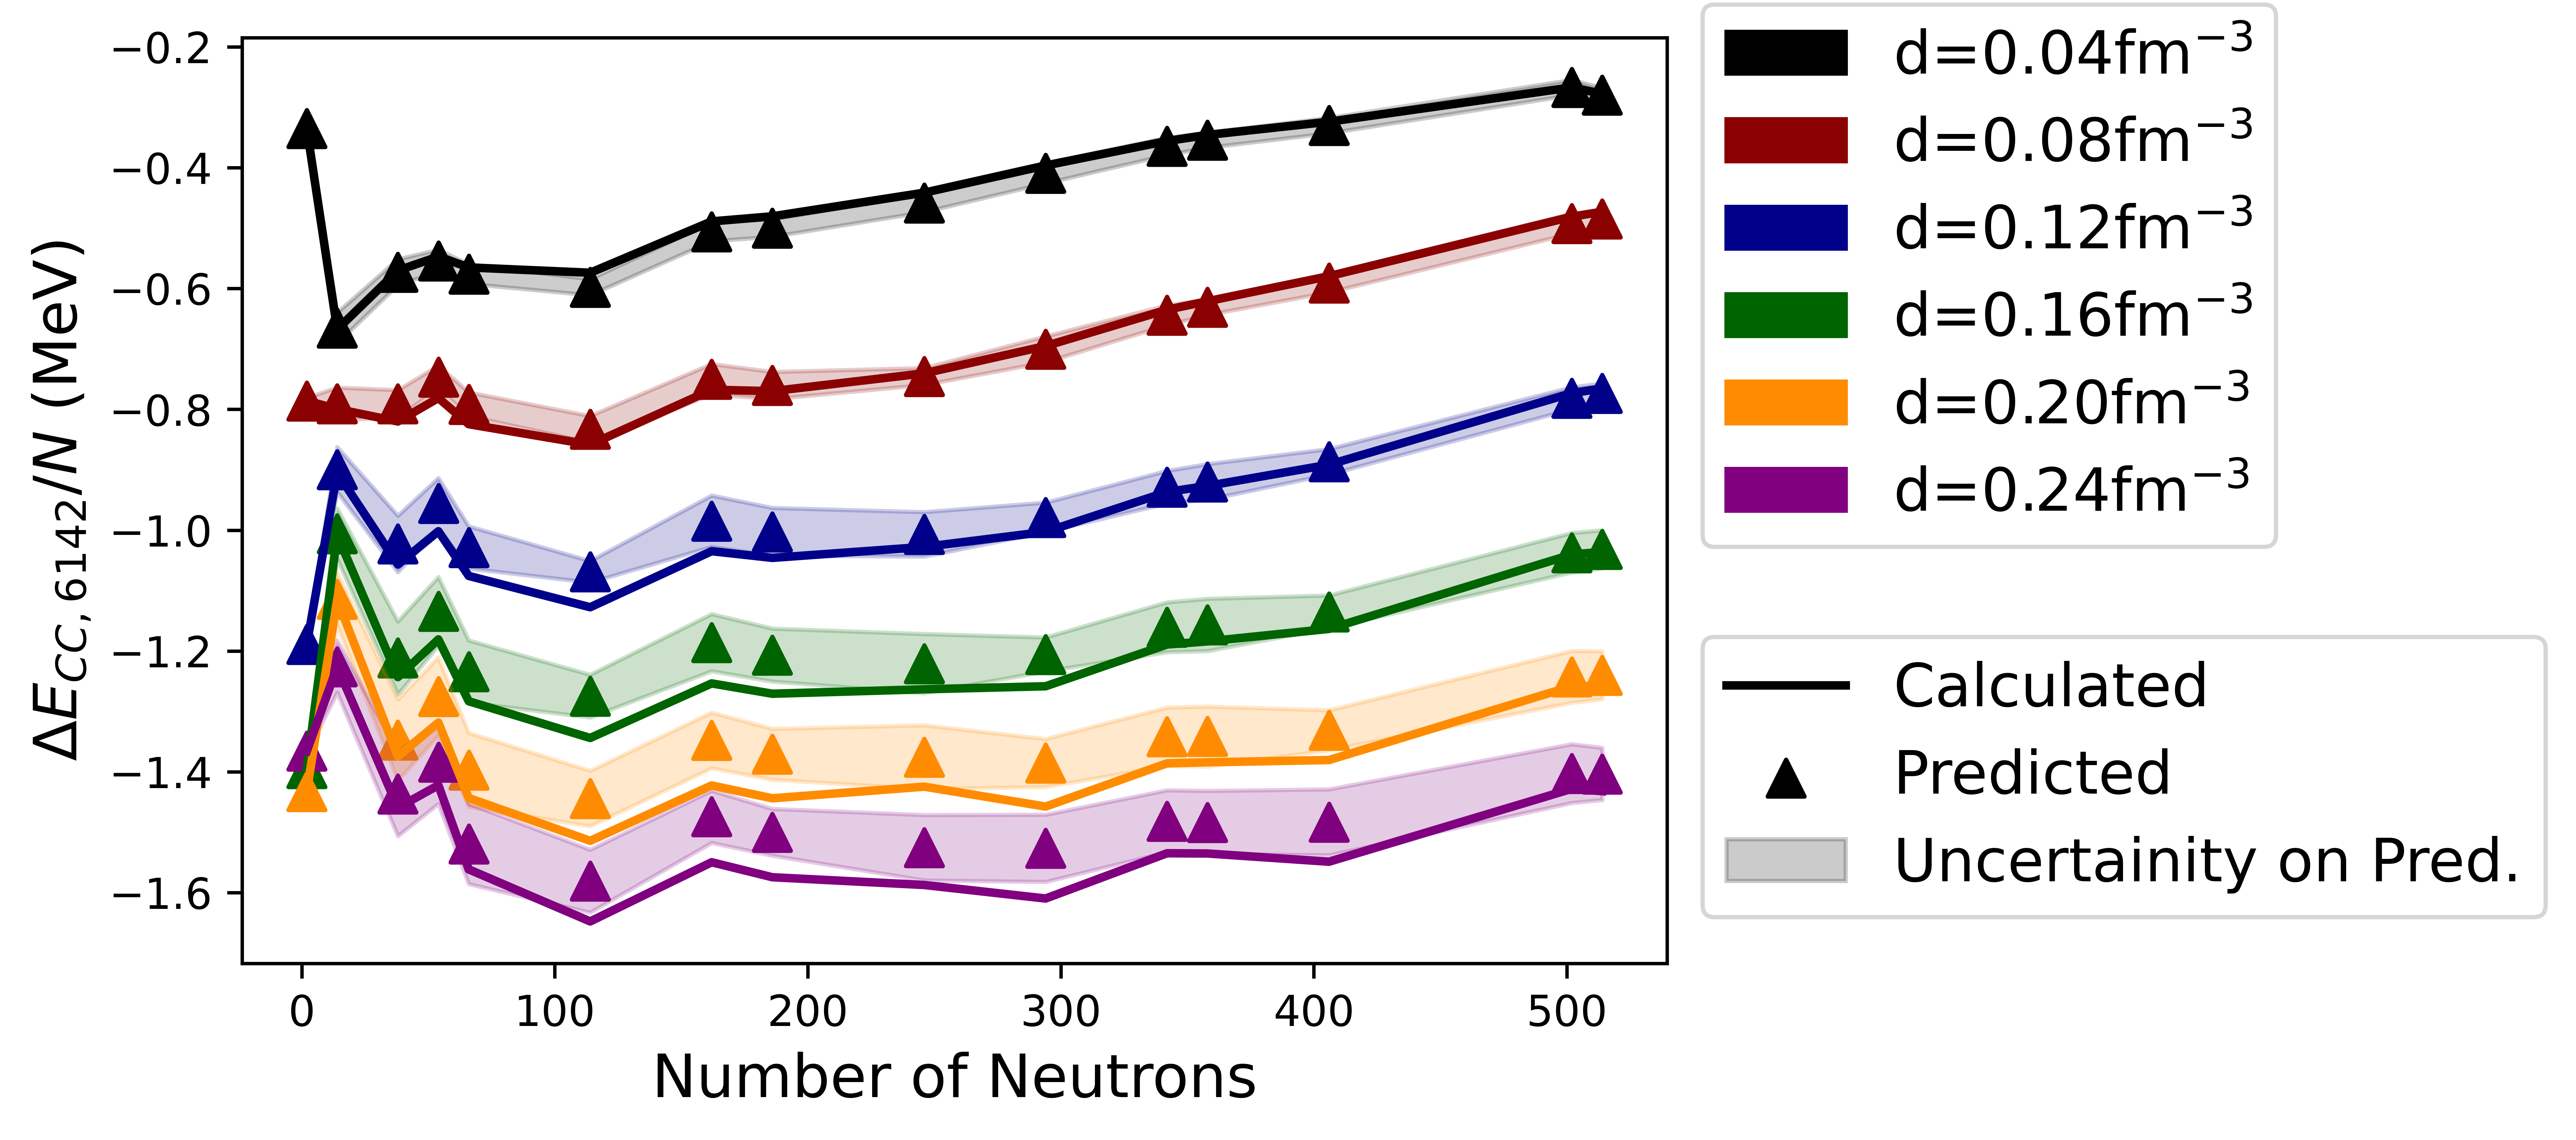
\includegraphics[scale=0.75]{Images/Chapter7/NeutronMatter/GP_PNM_MSU_n_1_uncertainity.png}
    \captionof{figure}{The CCD correlation energy per neutron as a function of the number of neutrons in the system for pure neutron matter with the Minnesota potential. All calculations are performed at 6,142 single particle states and with periodic boundary conditions. The full calculations, shown with the solid lines, were performed on MSU's ICER supercomputer. The SRE predictions, shown with the triangular data points, were predicted using only ten training data points from 5-14 open shells. The shaded region shows the Gaussian process uncertainty in predicting the converged correlation energy per neutron. The overall RMSE error between the full calculated and the predicted CCD correlation energies per neutron is 0.037 MeV.}
    \label{pnm_mp_all}
\end{center}

When looking at these results, it is also essential to consider the errors associated with other approximation schemes that do not involve machine learning—truncating the number of single-particle states in the system to some set number of energy shells. For example, if we limit the calculation to 14 open energy shells (15 to 30 shells), the error from the CCD correlation energies at 70 shells (M = 6,142) is 0.56 MeV, much larger than the GP result of 0.037 MeV. Furthermore, we can place include more energy shells before truncating. For example, if 40 total shells are included in the calculation, then the RMSE error from the results at 70 shells is 0.26 MeV; for truncating at 50 total shells, it is 0.15 MeV, and for truncating at 65 total shells, it is 0.045 MeV.  Therefore, even when exerting significant computational time and resources to raise the truncation level of the calculations, the GP prediction made with very little training data collected at a low number of energy shells is still the most accurate.

Accuracy is not the only metric we must consider; we must also consider the computational time and resources needed to generate the training data and perform the ML analysis versus just performing the complete calculation. The timing data presented in this paragraph was collected on Michigan State University's HPCC supercomputer on Intel Xeon processors with 2.40 GHz and 240 GB of RAM. The coupled cluster code was memory-optimized using the diagonal block structure developed in Ref. \cite{Ref5} and was parallelized using four compute nodes and 28 threads per node. Fig. \ref{pnm_mp_all} contains 90 points, each of which has to be individually calculated or predicted with the machine learning algorithm. Since each machine learning process has 15 points, 1,350 training points are needed to produce Fig. \ref{pnm_mp_all}.  However, their run times are comparatively short since they are from 5-14 open energy shells. Generating all 1,350 training data points takes 34.12 hours. It takes about 20 seconds to perform all 90 ML analyses, thus adding a negligible amount of time to the total ML analysis run time, which will be dominated by the time to generate the training data. To generate all 90 data points in Fig. \ref{pnm_mp_all} at 70 energy shells each, the total run time is 121.74 hours, meaning that by using the ML extrapolation method instead, 87.61 hours of computational run time is saved. That is equivalent to over 3.5 days of computational time saved and a resulting error of only 0.037 MeV!

It is possible to achieve better accuracy with this prediction method by changing the alpha hyperparameter of the Gaussian process algorithm. Instead of using the standard deviation of the training data as the alpha parameter (as used to generate Fig. \ref{pnm_mp_all}), instead we will use the fourth root of the standard deviation of the training data ($\alpha = \delta y_{train}^{1/4}$). However, while doing this increases the accuracy (the RMSE drops from 0.37 MeV to 0.25 MeV), the uncertainty drastically increases. As mentioned earlier, when working with these Bayesian algorithms, there seems to be a trade-off between the accuracy of the predictions and the size of the standard deviation of the prediction. The results for performing this extrapolation are shown in Fig. \ref{pnm_mp_all_n_0_25}, where the uncertainties are shown in (a) but are removed in (b) for clarity.

\begin{figure}[H]
\centering
\begin{subfigure}{0.48\textwidth}%
  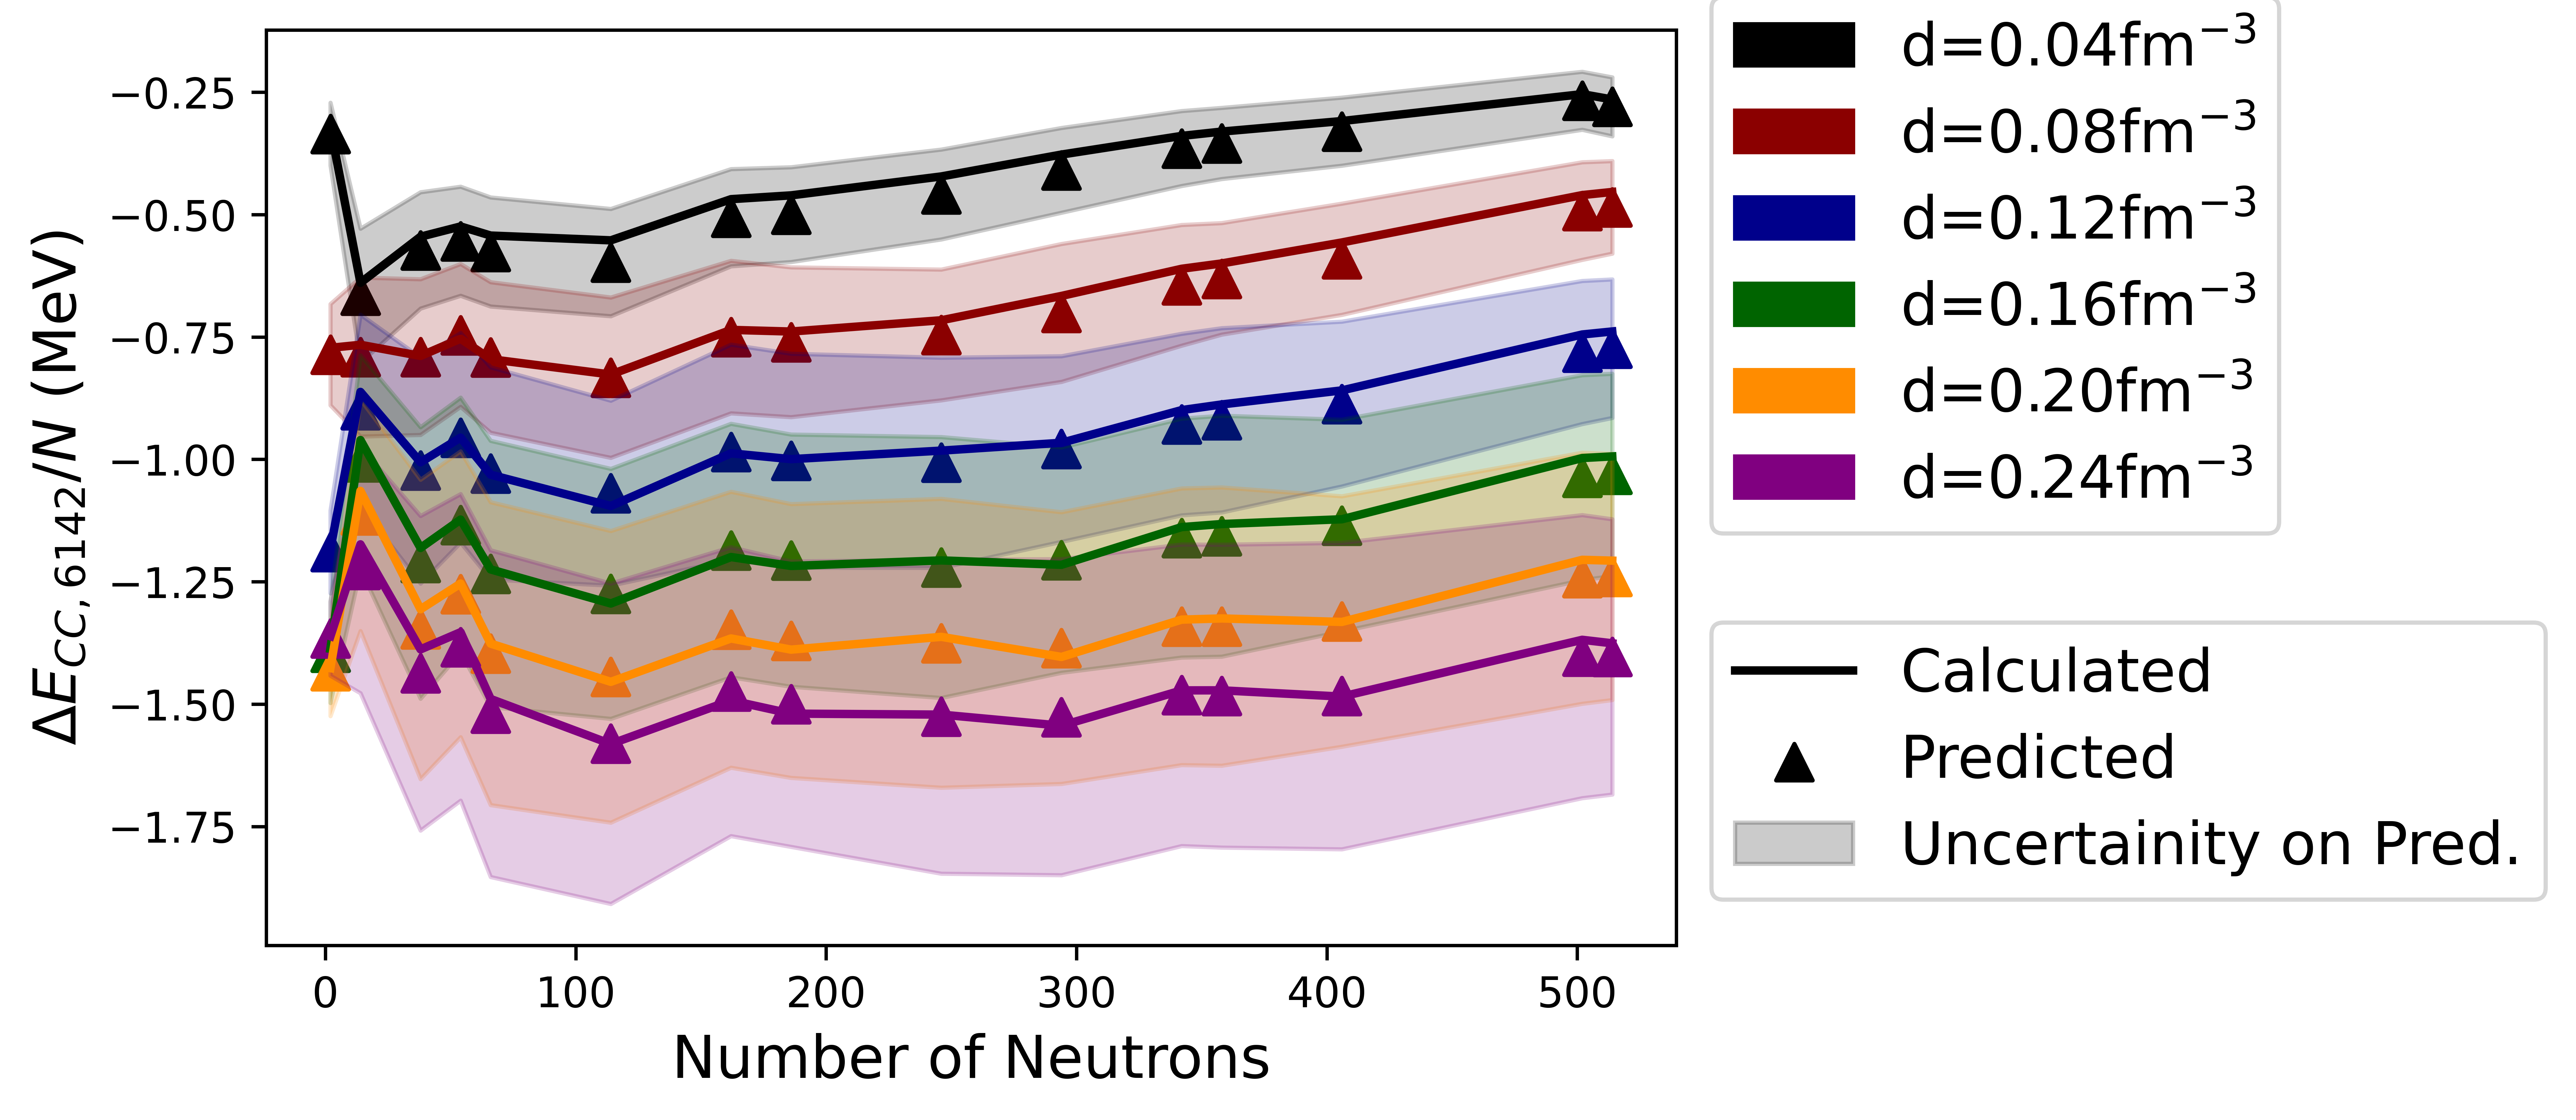
\includegraphics[width=\textwidth]{Images/Chapter7/NeutronMatter/GP_PNM_MSU_n_0_25_uncertainity.png}%
  \caption{A subfigure}
  \label{fig:sub1}
\end{subfigure}~%
\begin{subfigure}{0.48\textwidth}%
  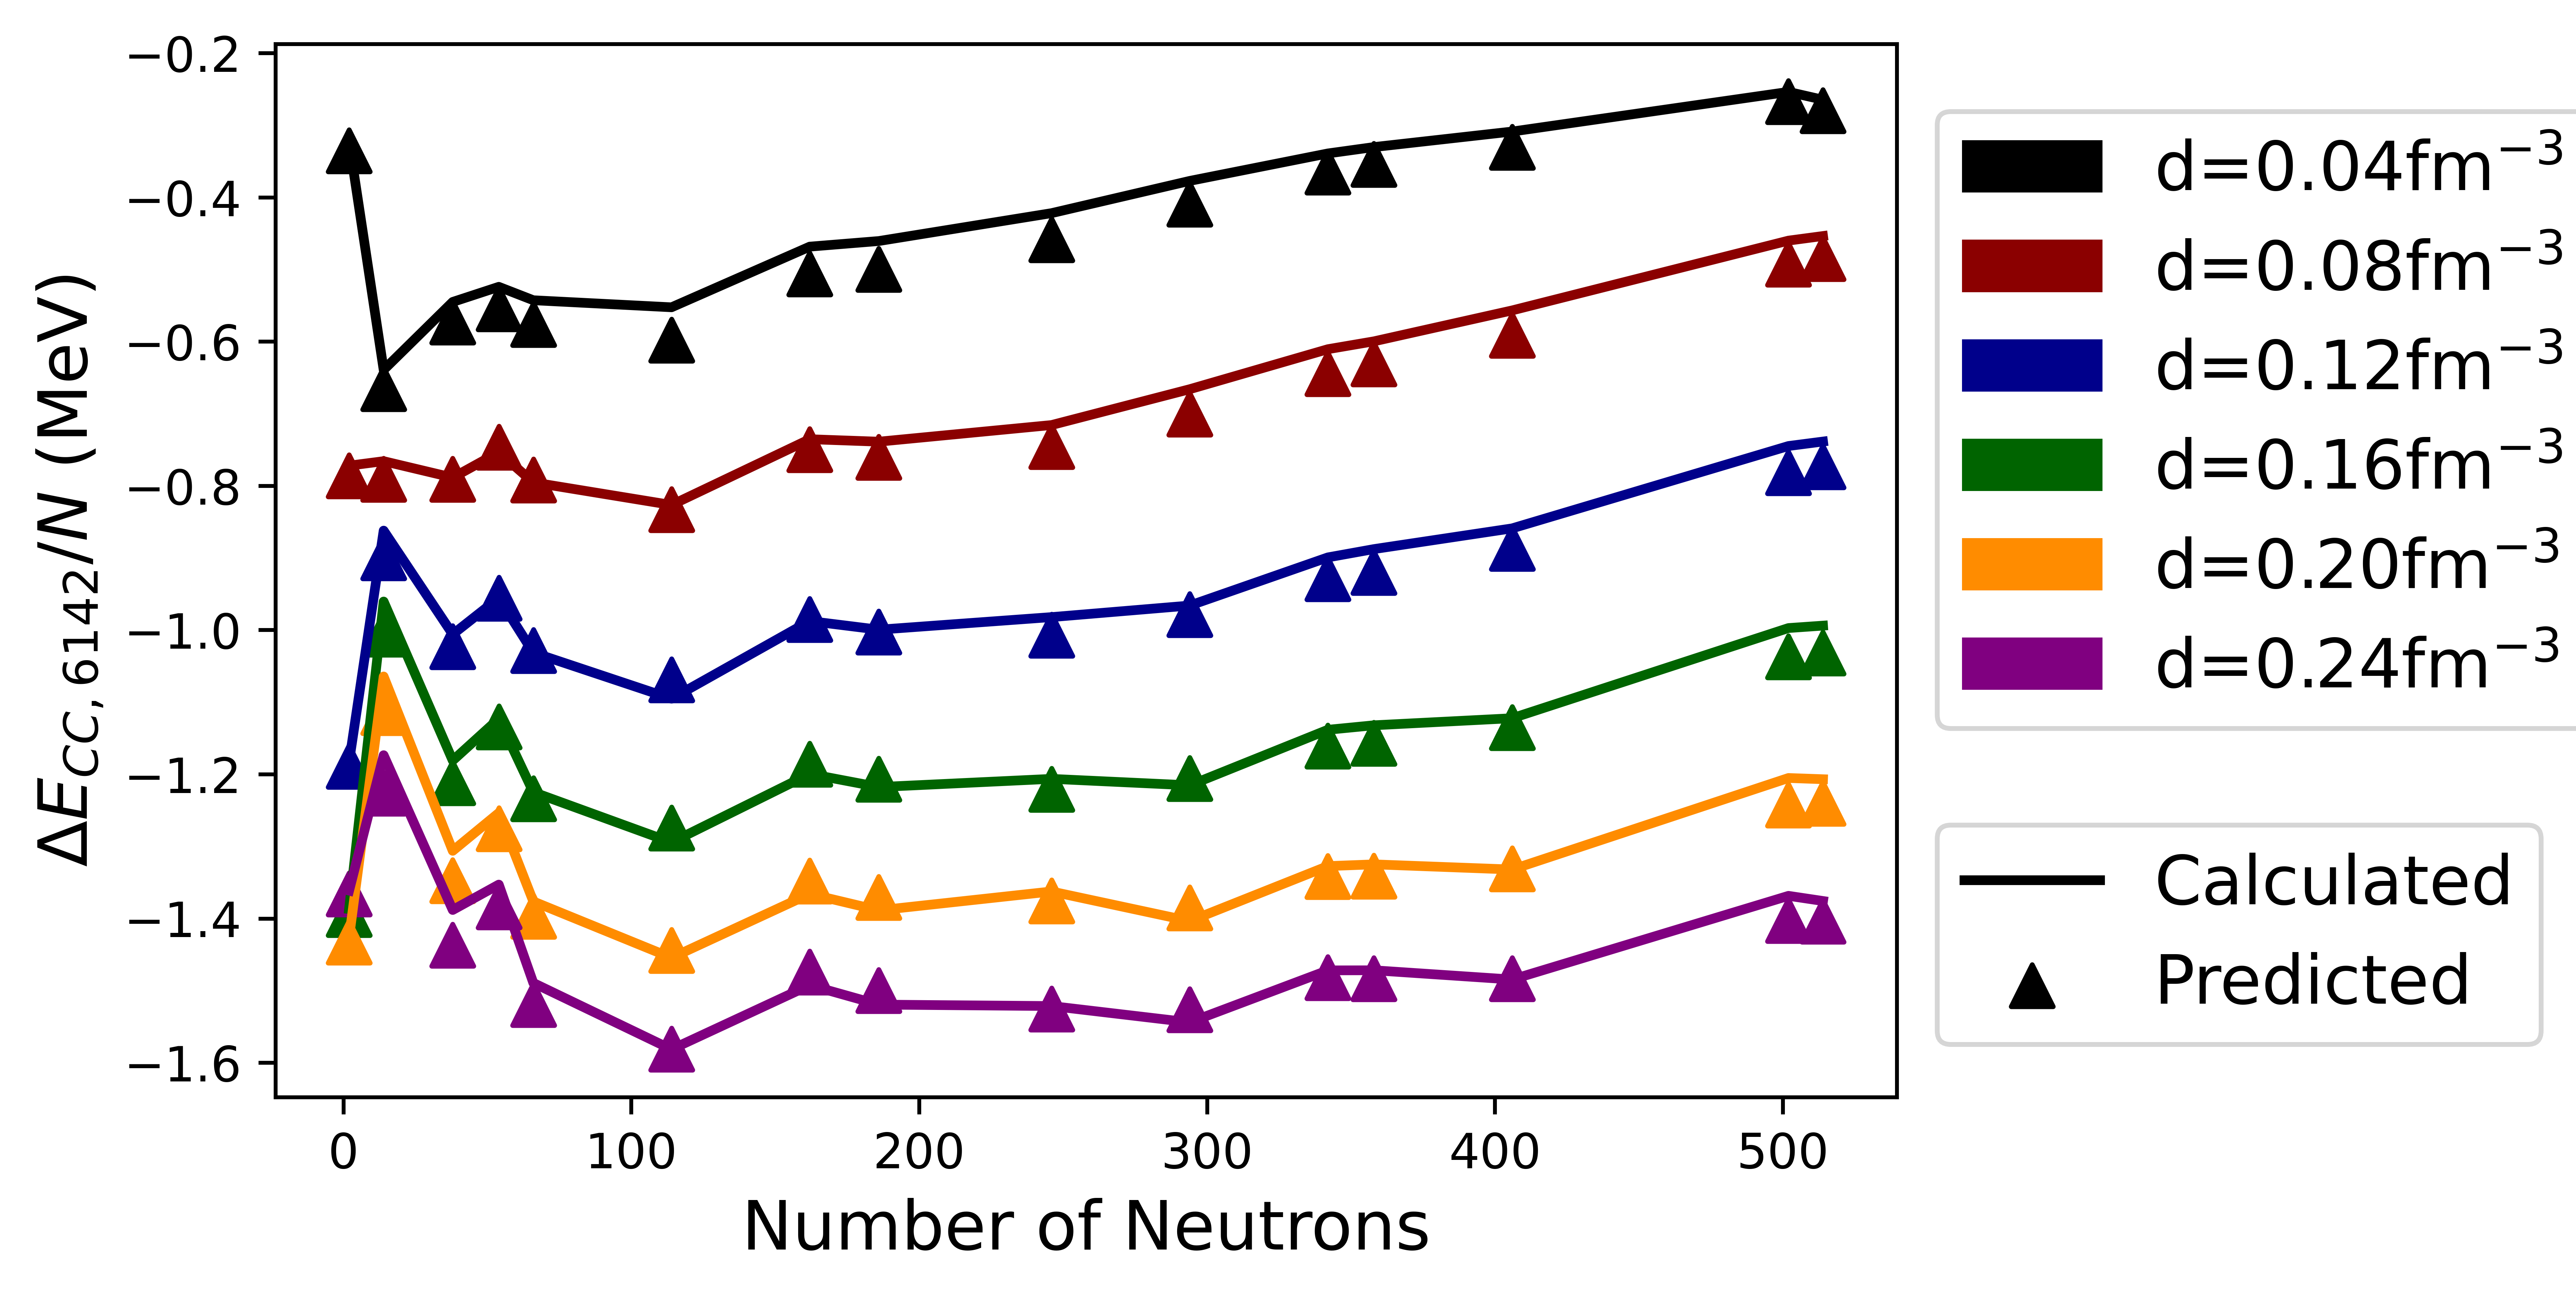
\includegraphics[width=\textwidth]{Images/Chapter7/NeutronMatter/GP_PNM_MSU_n_0_25.png}%
  \caption{Another subfigure}
  \label{fig:sub2}
\end{subfigure}
\caption{A figure with two subfigures}
\label{pnm_mp_all_n_0_25}
\end{figure}